\documentclass{article}

\usepackage{siunitx} % Provides the \SI{}{} and \si{} command for typesetting SI units

\usepackage{graphicx} % Required for the inclusion of images

\usepackage{tabularx} % Tables

\usepackage{natbib} % Required to change bibliography style to APA
\usepackage{float}
\usepackage{hyperref}


\usepackage{amsmath} % Required for some math elements

% Many options for pseudocode
\usepackage{algorithm2e}
\usepackage{algorithmic}

\usepackage{listings} % Python code blocks
\usepackage[margin=1in]{geometry} % CUSTOM

\setlength\parindent{0pt} % Removes all indentation from paragraphs

\title{Lab 3 Report: Wall-Following on the Racecar} % Title

\author{Team 22 \\\\ Benjamin Rich \\ Dinuri Rupasinghe \\ Sophia Wang \\ Steven Liu \\ Jose Soto \\\\ 16.405/6.4200} % Team # + Names, Class (RSS)

\date{\today} % Date for the report

\begin{document}

\maketitle


\tableofcontents
\newpage


\section{Introduction (Author: Dinuri Rupasinghe)}
% include a description of purpose and lab, define lab goals
% limit 6500 words. Short informal description of technical problem
The purpose of the wall follower lab is to make our racecar follow a wall and turn corners with safety controls in place. We are specified to utilize ROS software given by the course staff of Robotics, Science, and Systems. We will be utilizing the lidar sensor data we receive from the racecar to calculate distances of walls and objects to the car, the racecar router for transferring this data, and the wall follower package, which was given to us, in order to implement the Python scripts we will be creating.\\

The goals of this lab are to successfully have our racecar follow a wall, turn corners as required, and implement a safety controller that prevents the racecar from running into obstructions. We have designed a wall follower script and safety controller script to implement into our racecar workspace. These scripts were incorporated into our general wall follower node, which was also utilized in our lab 2 wall follower simulation. These scripts are important to our development of an autonomous system because we can give the system, in this case our racecar, a method to apply when they encounter specific situations and environments, such as following a wall or stopping when it is about to run into a person. This lab and the publishers and subscribers that we have implemented help us teach the racecar how to adapt to its current situation.\\

We tackle the technical problem by utilizing these main steps: implementing a PID controller, assuring that our car can accurately follow a wall with this PID control, adjust controls in order to handle corners and other wall anomalies, implementing a safety controller, and integrating and adjusting the software and hardware appropriately.\\

Using a slicing method, we will allocate fields of view for the front, left, and right views of the lidar sensor. By interpreting this data, our racecar is able to implement our PID control to determine where to adjust the angle of the wheels of the car in order to properly follow a given wall. \\

The challenge is that the lidar sensor is not robust to noisy data. We approach this technical challenge by implementing a least squares regression for our distance data. After implementing our safety controller and wall follower script, our racecar successfully completed the goals of this lab.\\






\section{Technical Approach (Author: Benjamin Rich)}

\subsection{Overview}
Our technical approach to this lab occurred in the following steps: 
\begin{enumerate}
    \item Implement a PID controller. 
    \item Implement wall following using the PID controller. 
    \item Make wall following more robust by handling corners.
    \item Implement a flexible safety controller.
    \item Make adjustments to fine tune software-hardware interface. 
    \item Test entire system as a package. 
\end{enumerate}
Much of the code for the PID controller and for wall following comes from Ben R's Lab 2 Wall Following code, although it was greatly improved for robustness and team code reviews caught and fixed several bugs. 

\begin{figure}[h]
\begin{center}
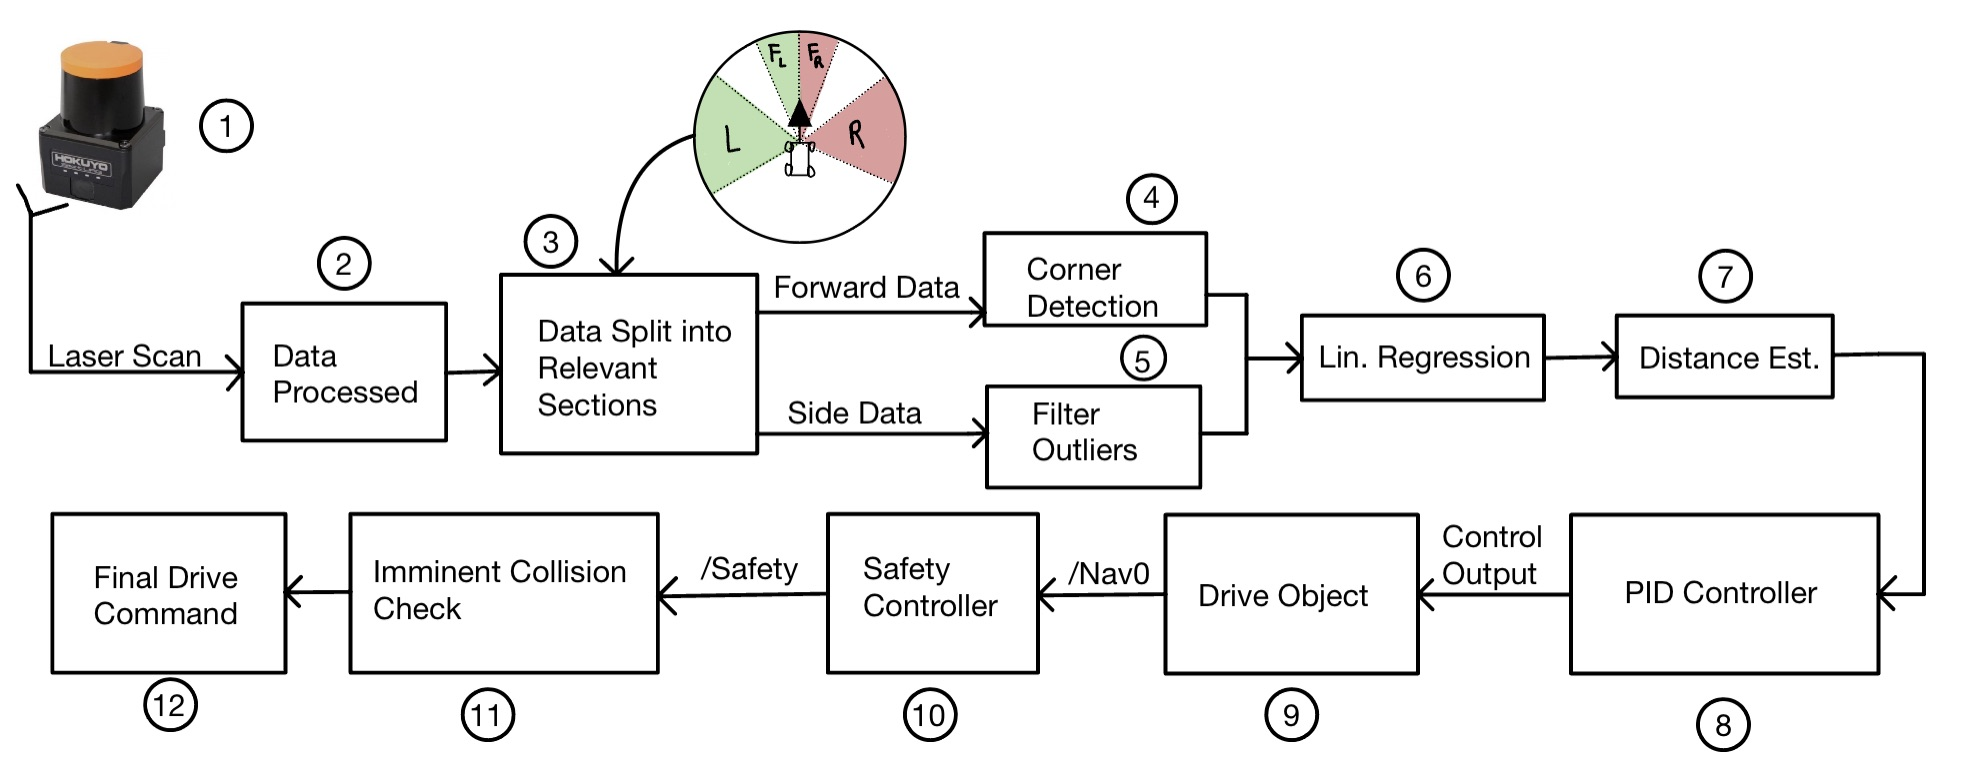
\includegraphics[width=0.85\textwidth]{DataFlowImg.png} % Include the image placeholder.png
\caption{Simplified Wall Follower and Safety Controller Workflow for One Laser Scan Output}
\end{center}
\label{workflow}
\end{figure}

As shown in Figure 1, our wall-follower code listens to outputs from our Hokuyo 2D Lidar. This data is processed and sliced, outliers are removed, a line is fit to relevant data, and corners are identified if present. The data is then passed to a controller class which, when given an estimated distance from the wall, returns a control output to reduce error with minimal overshoot and settling time. The output from our PID controller class is then written to a drive object, and published via a nav topic. This drive object is then intercepted by our safety controller, which also listens to the laser-scan data. Our safety controller checks for an imminent collision, and if so, stops the car immediately. Depending on user inputs, a minimum amount of time for the car to stop can be specified. \\




\subsection{PID Controller}
In order to have robust wall following code, we required a controller that is robust to disturbances. One solution is feedback control. PID (Proportional Integral Derivative) Control is a common and effective method of developing a feedback controller with minimal overshoot, minimal settling time, and relatively fast rise time. A general block diagram implementation of a PID controller is shown in Figure 2. 

\begin{figure}[h]
\begin{center}
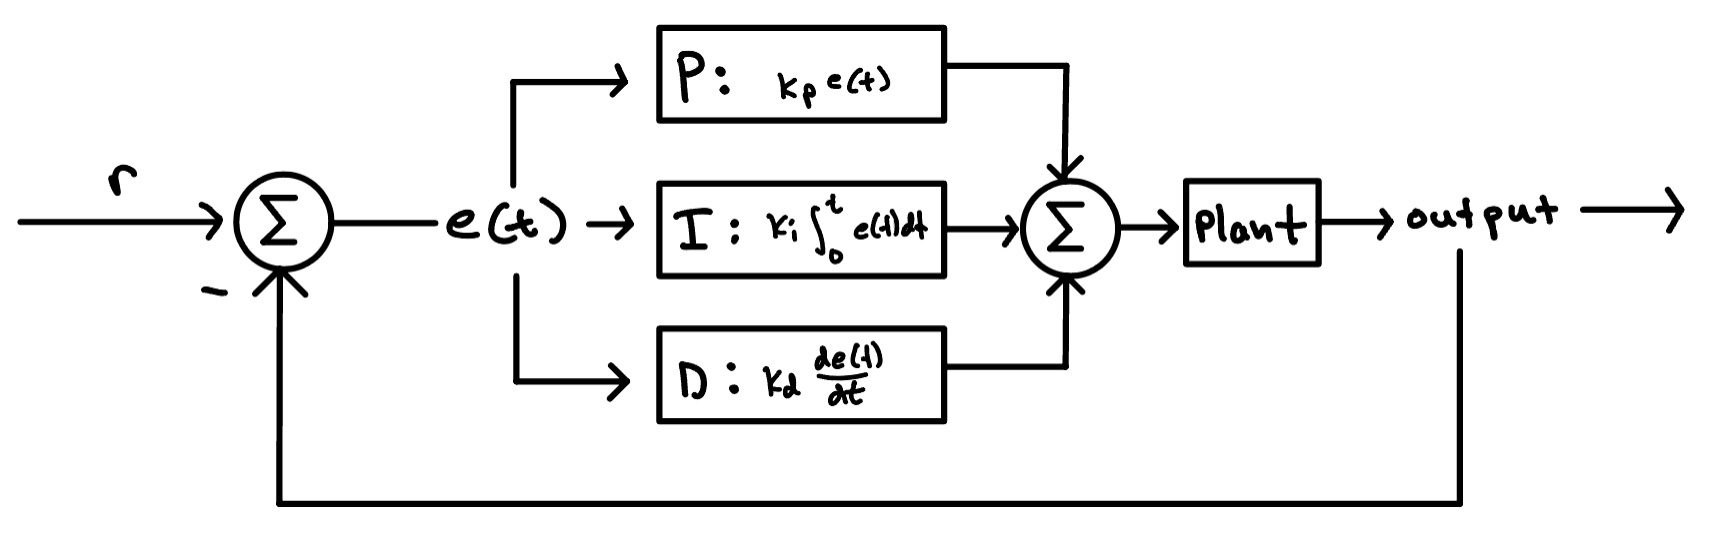
\includegraphics[width=0.7\textwidth]{pidblockdig.png} % Include the image placeholder.png
\caption{Data Slicing Sections}
\end{center}
\label{workflow}
\end{figure}

We created a basic PID Python class to handle storing previous error, input, output, and time data, which can accept function calls with an estimated distance from wall and return a control output to minimize error (see Appendix A: PID Class Code). Our controller stores values and, when called, uses the following formula to calculate our control output:

\begin{equation}
    u(t)=K_pe(t)+K_i\int_0^te(\tau)d\tau + K_d\frac{de(t)}{dt}
\end{equation}
Here, $u(t)$ is our control output, $K_p$ is our proportional gain, $K_i$ is our integral gain, $K_d$ is derivative gain, and $e(t)$ is our error with respect to time (calculated by $position(t)-setpoint$). $K_i, K_p, \textrm{and } K_d$ are chosen through iteration, which will be discussed more in further sections. In practice, we must perform a discrete approximation of (1), as we cannot perform integration when we have discrete data. So, our code performs a 1-time-step trapezoidal integral approximation. That is, we use the formula:
\begin{equation}
    u(t) = K_p*e(t_{1})+K_i*\frac{(e(t_1)+e(t_0))}{2}*(t_1-t_0)+K_d*\frac{e(t_1)-e(t_0)}{t_1-t_0}
\end{equation}
where $t_1$ is the current time, and $t_0$ is the previous time that the PID controller was called. After this formula is calculated, $t_0$ is updated to equal $t_1$, and $e(t_0)$ is updated to equal $e(t_1)$. The control output $u(t)$ is then returned. Often, multiple timesteps are integrated (i.e. more than one timestep is stored), however, we found one timestep to be sufficient for stable yet reactive control.


\subsection{Wall Following}
Upon implementing a PID controller, we could now implement a basic wall following method. Wall following has several key parts: (1) data selection and slicing, (2) filtering, (3) wall and corner detection and avoidance, (4) least squares regression and distance estimation, (5) call to PID and Publishing.\\

\textbf{\underline{Data Selection and Slicing}}: 

Our wall following node is initialized with a subscriber to $/scan$, which listens to the output from our Hokuyo Lidar. Data is received from $/scan$ as a LaserScan message which contains various data including the minimum angle of scanning $(\theta_{min})$, maximum angle of scanning $(\theta_{max})$, angle increment ($\delta_{\theta}$), and the laser scan distance values ($arr$). We first process data by iterating from $\theta_{min}$ and $\theta_{max}$ to pair each disance in $arr$ with its angle relative to the car, generating $arr' = [(dist_1,\theta_{min}),....,(dist_n,\theta_{max})]$. We then remove any values with $\theta < -120\deg$ or $\theta > 120\deg$ (we only want to look somewhat behind the car). We then slice our data into useful chunks using the formula (in Python notation)
\begin{equation}
    ({R,R_F,R_L,L}) = (arr'[0:3*p],arr'[int(4.5*p):5*p],arr'[5*p:int(5.5*p)], arr'[7*p:])
\end{equation}
where $p=len(arr')//10$. Because the Hokuyo Lidar returns data from the right of the robot in the front of $arr$, and scans counterclockwise to the left of the robot, this method returns 4 chunks of data, $R,F_R,F_L,L$, whose positioning is shown in Figure 3. \\

\begin{figure}[h]
\begin{center}
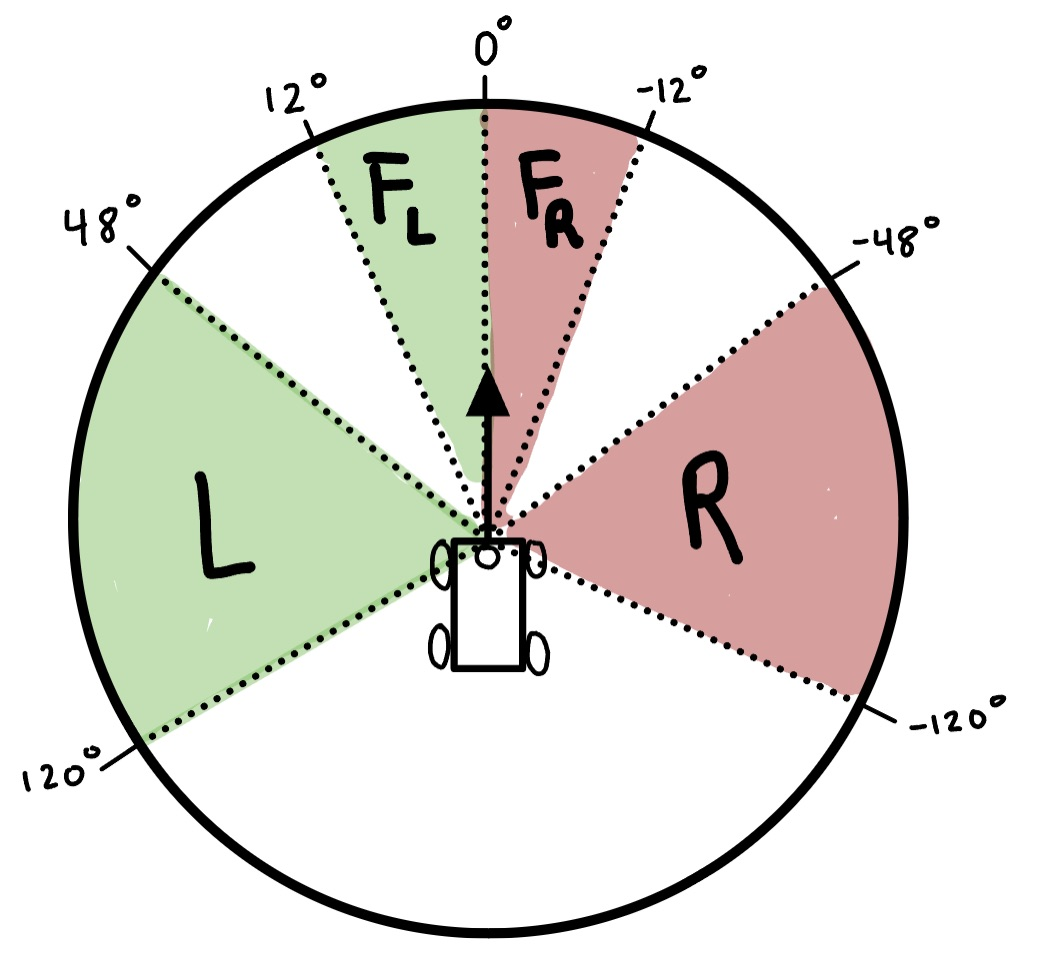
\includegraphics[width=0.4\textwidth]{Splicing.png} % Include the image placeholder.png
\caption{Data Slicing Sections}
\end{center}
\label{workflow}
\end{figure}

This slicing method is selected based on the logic we need to follow walls and tuned based on practical performance. With $0\deg$ defined as the front of the robot, and $-90\deg$ as the right of the robot, we choose ranges such that our $L,R$ sections are mostly directly the side of the robot, but some data slightly behind the robot (which helps later on with outward corners) and some slightly ahead is included to help reduce error from a noisy sideways wall reading. A small range is used for forwards data so that we can look ahead to the left, and ahead to the right, allowing for corner detection.\\

\textbf{\underline{Filtering}}: 

We perform filtering on our $L,R$ data. This is a necessary action and we found it to drastically improve the robustness of our wall following algorthim. There are a number of unique circumstances where removing outlier datapoints is useful; for example if part of a wall is see through (i.e. some distances returned might be much larger than reality), or if part of a wall is missing, or if you receive noisy wall scans. Several filtering methods were tested, including filtering about the $avg$, but filtering about the $minimum$ distance was found to be the most effective. In our code, we filter $L,R$ data by removing any data that is more than $\gamma$ (a constant) times the minimum value in $L,\textrm{and }R$ respectively.\\

\textbf{\underline{Wall and Corner Detection and Avoidance}}

We first decide which data chunks to use. If we are following the right wall (which we check by by loading a parameter), we use $R,F_L$, and for a right wall we use $L,F_R$. To maintain generalizability, call these pairs $S,F$ where $S$ is the side section and $F$ is the forward opposite side section. If $avg(F)<threshold*setpoint$, we consider ourselves at an inside corner, where $threshold$ is some constant (we used 2.0), and setpoint is our desired distance from the wall. Then, we code for three different cases:
\begin{enumerate}
    \item The robot is next to a wall that continues without an inside or outside corner. 
    \begin{itemize}
        \item $avg(F)>threshold*setpoint$; the car is not approaching an inner corner. So, only pass $S$ data to least squares regression.
    \end{itemize}
    \item The robot is next to a wall that is approaching an inner corner. 
    \begin{itemize}
        \item $avg(F)<threshold*setpoint$; the car is approaching an inner corner. In this case, we need to react to a corner! We pass both $S$ and both $F_R$ and $F_L$ data (we concatenate these three sliced sections) to least squares regression, and we set $Corner=True$ (this will be used in our call to PID). The data is concatenated so that as a robot goes along an inner corner, the fitted line from least squares regression is diagonal w.r.t. the corner as expected. 
    \end{itemize}
    \item The robot is next to a wall that is approaching an outer corner. 
    \begin{itemize}
        \item $avg(F)>threshold*setpoint$; the car is not approaching an inner corner. Our call to filtering on $S$, upon passing the beginning of the outer corner, will filter out data that is not from the other side of the outer corner. In other words, our filtering method accounts for outer corners, by accurately choosing to only keep points close to the robot! We thus just pass $S$ to least squares regression. 
    \end{itemize}
\end{enumerate}






\textbf{\underline{Least Squares Regression and Distance Estimation}}

We perform least squares regression on our data to produce a point as our estimated distance from the wall. This involves converting $(dist,\theta)$ to $(x,y)$ values and performing least squares regression on these values. Least squares regression finds a line of formula $\hat{y}=a+bx$ where $\hat{y}$ minimizes the difference between observed values (our data) and the values a model outputs. In our code, we perform linear least squares regression using numpy methods and return estimated distances from the fitted line. We then choose the minimum estimated distance and consider this as distance from the wall. \\

\textbf{\underline{Call to PID and Publishing}}

Using our estimated distance from the wall, we can now make a call to our PID class to receive a control output. However, in order to account for inside corners, we first, if $Corner=True$ (i.e. we are at an inside corner), subtract $constant\_offset$ from our estimated difference. This has the effect of making the control react rapidly and earlier than it otherwise would. If we visualize how a robotic car might approach making a 90-degree turn, this makes sense. \\

\begin{figure}[h]
\begin{center}
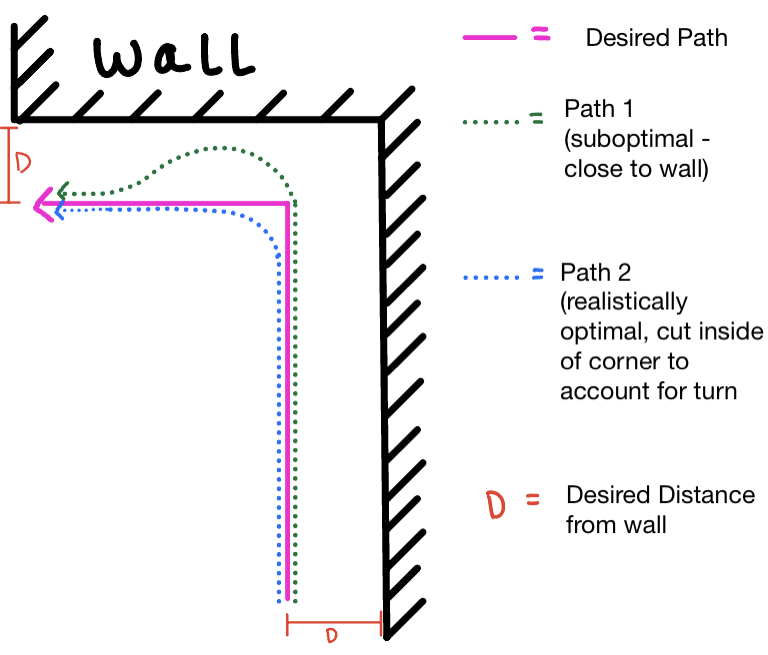
\includegraphics[width=0.45\textwidth]{TurnImg.png} % Include the image placeholder.png
\caption{Illustration of Car Turning for Inside Corner}
\end{center}
\label{turning}
\end{figure}

As shown in Figure 4, if we start turning only once the car detects it is getting too close to the wall (i.e. once the estimated distance is less than desired distance; path 1), due to the turning radius of the car, it would wind up very close to the wall. Instead, our team uses the method of path 2; we send a signal to our PID class that makes the control law 'think' that we are closer to the wall than we truly are once at a corner, making the car react a bit prematurely to 'cut the corner' as shown in Figure 3. As it turns the corner, it stops sensing a corner, and unmodified estimated distance is then used again. This method proved very effective during testing. \\

The output from our PID class is a control output which we then write to an AckermannDrive object, and publish to $/nav0$. This concludes one execution of our wall follower script! Our implementation is displayed in Appendix B: Wall Follower Code. 


\subsection{Safety Controller (Author: Steven Liu)}

Our safety controller is relatively simple in execution. The safety controller node subscribes to both $/scan$ for LIDAR scan data and the high-level $/vesc/high\_level/ackermann\_cmd\_mux/output$ topic in order to intercept the drive commands published by the wall follower node. Each of these subscribers has an associated callback function, \\

When data is received from $/scan$, we use similar slicing techniques to those used to conduct the wall following in order to determine how close obstructions are in front of the car. In particular, we find the minimum of 
\begin{equation}
    arr[int(0.4*len(arr)):int(0.6*len(arr))]
\end{equation}
where $arr$ is the array of ranges returned by the lidar scan. This is stored in a variable $min\_dist$ in order to keep track of how much clearance the robot has in front of it nearly in real time. \\

Drive data received from $/vesc/high\_level/ackermann\_cmd\_mux/output$ is intercepted, and a check is conducted to determine if the car should be stopped. This consists of two conditions.
\begin{equation}
    min\_dist < 0.15*data.drive.speed+0.3
\end{equation}
where $data$ is the attempted wall follower command, then the car should stop. The coefficients here were determined experimentally; the constant term provides a minimum buffer of space to account for the bumper and allowing for some margin of safety, while the linear term accounts for the fact that a faster-moving car will take longer to stop. \\

The other condition is if it is within $pause\_time$ seconds of when the last stop command was issued, such that the car will stop for a minimum of $pause\_time$ when it does stop. This is done by setting a flag $paused$ when the car is ordered to stop and the $paused$ flag is not already set, recording the time so it can be unset $pause\_time$ seconds later. \\

If the car is to be stopped, a command is published to $/vesc/low\_level/ackermann\_cmd\_mux/input/safety$ with drive speed set to zero, overriding the original command and stopping the car. Otherwise, if both checks pass, the original drive command is passed along as-is, allowing the car to continue as planned.



\subsection{Adjustments for Hardware: Putting it all Together}
Although we were able to test some of the code in Lab 2, modifications were needed to make our wall following robust enough to operate well on the physical car. \\

In particular, significant tweaking of PID gains was required to find gains that worked well at different speeds and different terrains. Ultimately, through iteration, we settled on the gains below so that the car responds quickly, but is stable with minimum overshoot.
\begin{equation}
    K_p = 1.0\hspace{10mm} K_d = 0.13 \hspace{10mm} K_i = 0.1
\end{equation}


Additional iteration was performed to determine constant factors in our code such as $\gamma, corner\_threshold,$ and $constant\_offset$, which refer to the multiplier of minimum distance above which we filter out values, the multiplier of desired\_distance which when on average the front values are below then we consider the car at a corner, and the amount our estimated distance is manipulated when at a corner, respectively. Our final values are shown below.
\begin{equation}
    \gamma = 2.0 \hspace{10mm} corner\_threshold = 2.5 \hspace{10mm} constant\_offset = 0.5
\end{equation}
In summary; through iteration, we refined the constants used in our model and ensured that all components worked together in unison. 


\section{Experimental Evaluation (Author: Sophia Wang)}

Our racecar was tested numerous times to guarantee robustness. Although many tests were performed, we recorded and processed data for 5 unique tests at 5 different locations in the basement of MIT Stata Center. In this section, we present a performance evaluation based on field experiments.\\

Four parts of our system are evaluated and discussed: wall following, corners, noise, and safety controller. For each test, we recorded the car's distance from the wall. In our figures, we show the desired distance from the wall as well as a $\pm 20\%$ error margin. \\

\subsection{Manual Driving and RVIZ}
Before implementing wall following, we first ensured that we could manually control our car through a controller, and visualize laser scan data in RVIZ, s shown in Figure 5. Visualizing laser scan data proved valuable while transitioning from software to hardware. 

\begin{figure}[H]
\begin{center}
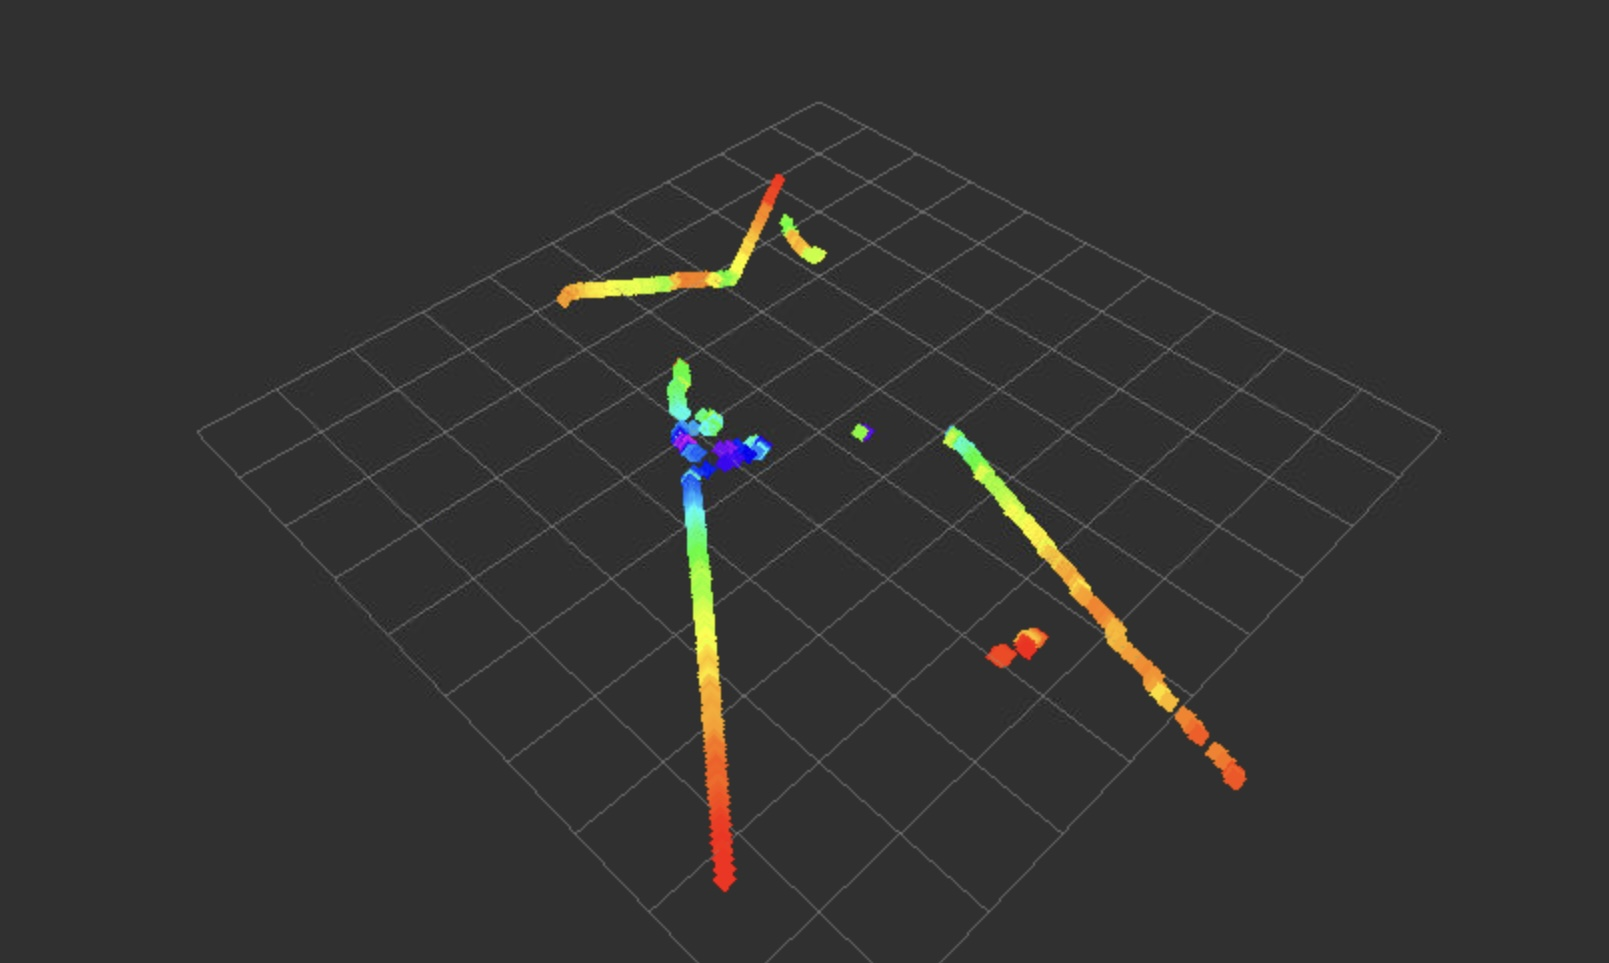
\includegraphics[width=0.6\textwidth]{rviz scn.jpg} % Include the image 
\caption{Example RVIZ Laserscan Visualization}
\end{center}
\label{workflow}
\end{figure}

\subsection{Wall Following}
We began by testing our system on a wall without any curves or corners with a moderate speed of 0.5 meters/second and a desired distance of 0.5 meters from any detected surface. The choice to follow a right wall as opposed to a left wall was largely arbitrary, as we demonstrate left following functionality in future tests. The car was manually angled from the wall before the autonomous system was activated. As shown in Figure 6, within ~3 seconds of activation, the PID controller corrected the car navigation to the desired distance and continued maintaining this distance for all time after. Throughout this simple wall following test, we never exceed a $\pm 20\%$ error margin.\\

\begin{figure}[H]
\begin{center}
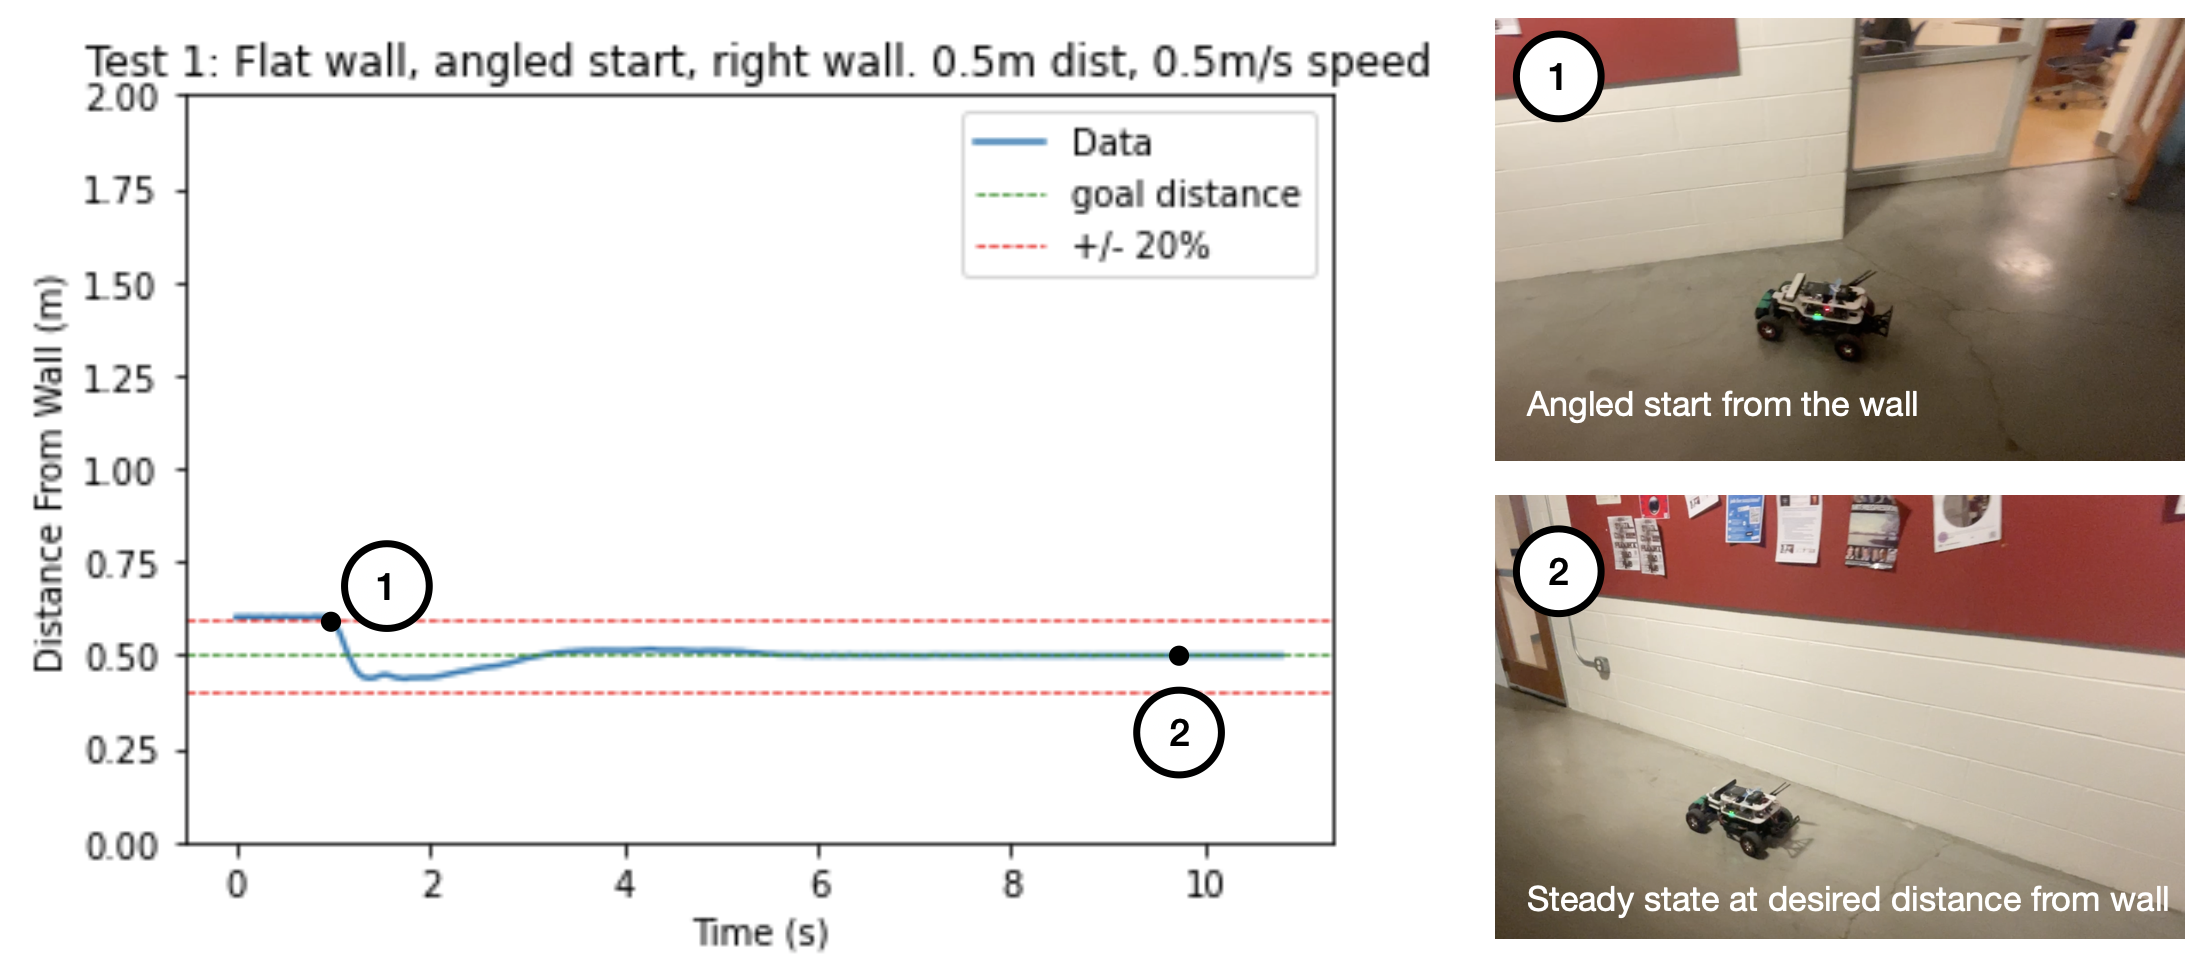
\includegraphics[width=0.7\textwidth]{wall_follower_figure.png} % Include the image 
\caption{Wall Following: Straight Wall}
\end{center}
\label{workflow}
\end{figure}

\subsection{Corners}
We were interested in testing two types of corners: outer and inner. An outer corner is where the corner projects outward into an open space, whereas an inner corner is defined as when two walls meet and project into a corner. Our first test with a complex multi-corner starts with an outer corner, then quickly turns into an inner corner. We maintained previous default settings of right wall following, a speed of 0.5 meters/second, and a desired distance of 0.5 meters. As shown in Figure 7, when the car begins the outer and inner corner turn, the robot's distance from the wall is overshot by around 20\%. Additionally, we found no significant difference between the car's performance on inner and outer corners.

\begin{figure}[H]
\begin{center}
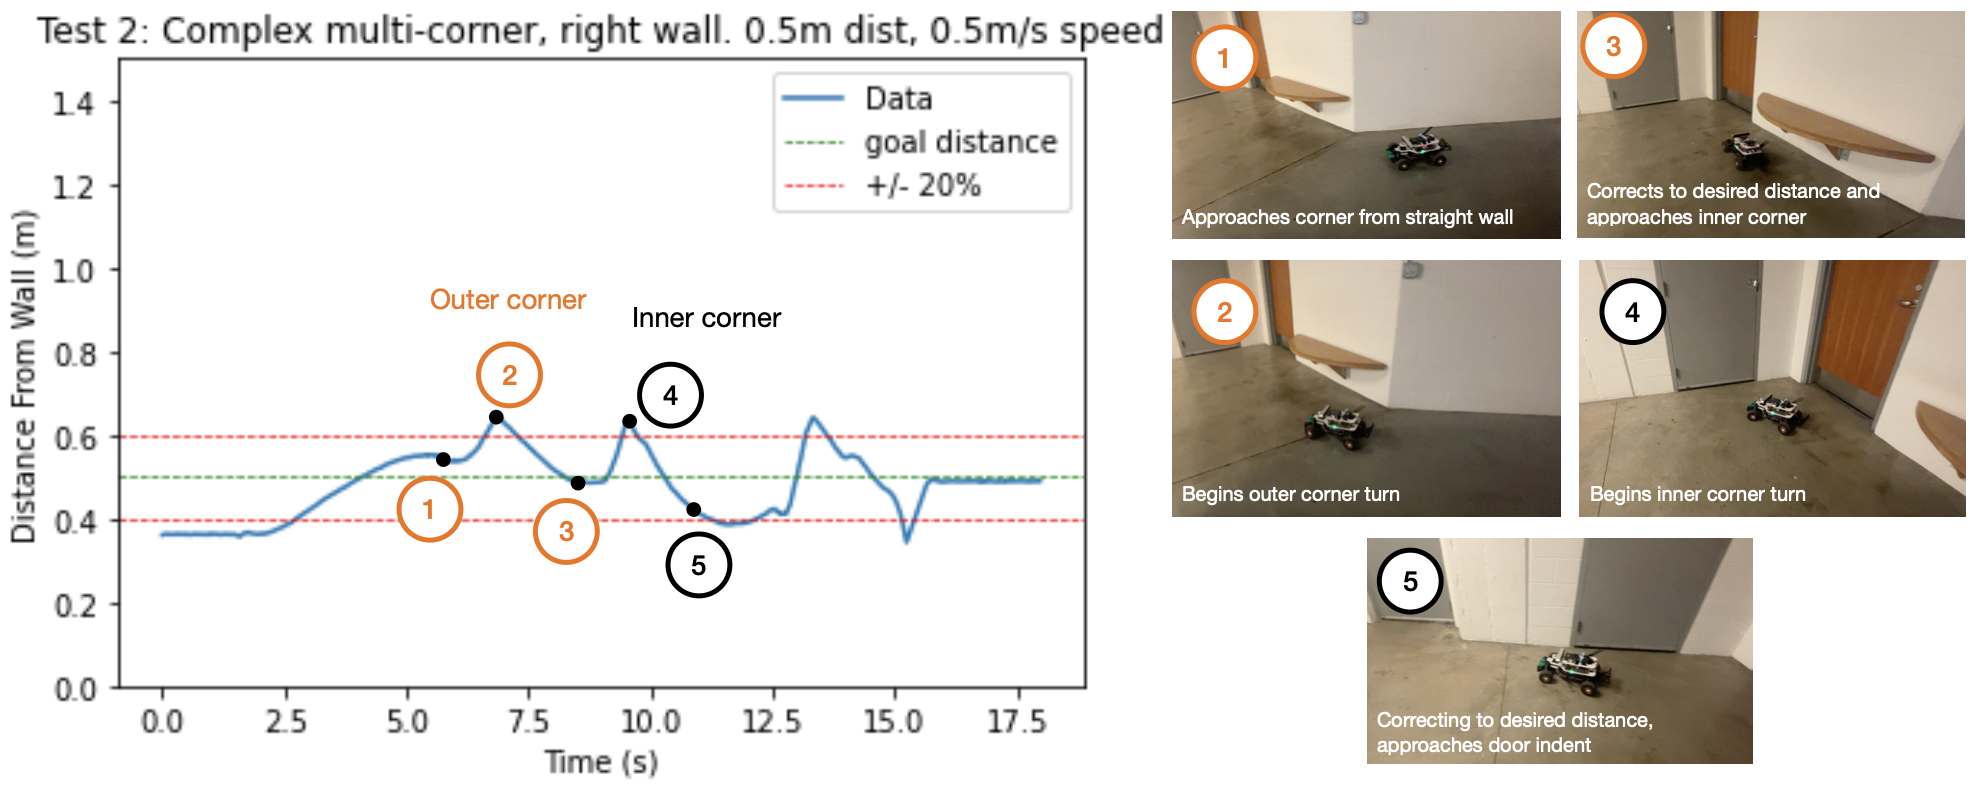
\includegraphics[width=0.85\textwidth]{corners_figure.png} % Include the image placeholder.png
\caption{Right Wall Following: Inner and Outer Corners}
\end{center}
\label{plot}
\end{figure}

In our second corner test, we again found a sequence of a contiguous wall with an outer then inner corner. Here, we kept the same settings but changed to left wall following. As shown in Figure 8, we again observed an overshoot when beginning steering a turn. This offshoot was larger than that observed when right following (we overshot by around 30\%), which could possibly be explained by the crowded presence of ourselves and other teams in the hallway when testing. This could have interfered with the laser scan data from which our system draws navigation commands. In this test, we observed our first undershoot of desired distance, where our car approached the wall too closely. This occurred after the robot completed the inner turn at around a 30\% error margin from our desired distance. Interestingly, this test ended in the activation of the safety controller when the car detected an obstacle, an incoming pillar. We discuss the performance of the safety controller in a later section.\\

\begin{figure}[H]
\begin{center}
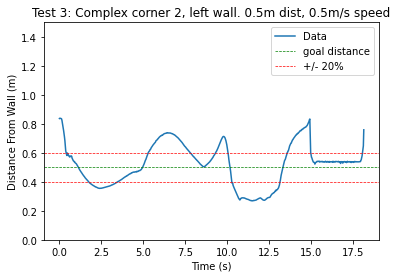
\includegraphics[width=0.5\textwidth]{plot3.png} % Include the image placeholder.png
\caption{Left Wall Following: Inner and Outer Corners}
\end{center}
\label{workflow}
\end{figure}

Our last corners test was at the following settings: right wall following, a speed of 1.5 meters/second, and a desired distance of 1.5 meters. At higher speeds, our car is more oscillatory with higher error at around 20\% overshoot when beginning a turn, as shown in Figure 9. We observe more oscillations because the real-world physical system can't change its state instantly. While the controller may be near the target of the wall, it takes some time for the PID controller to correct its proportional feedback. Because we are operating the system at three times the speed of previous tests, during this time, the system approaches even closer to the wall. By the time we introduce the proportional feedback, we  then need to adjust our derivative control to address our undershoot. This back-and-forth correction results in oscillations. The test demonstrated our system's vulnerability to high speed operation.\\

\begin{figure}[H]
\begin{center}
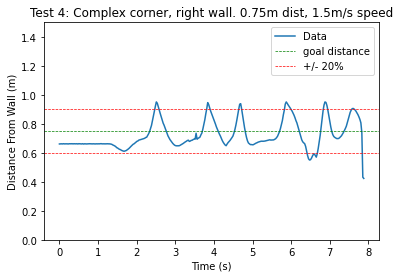
\includegraphics[width=0.5\textwidth]{plot4.png} % Include the image placeholder.png
\caption{High Speed Wall Following: Inner and Outer Corners}
\end{center}
\label{workflow}
\end{figure}

\subsection{Noise}
The last of our five tests addressed noisy walls. Previous tests were performed on uniform surfaces (e.g. the concrete walls of the basement). For this test, we ran the car alongside a bumpy "wall" composed of wooden crates, cloth surfaces, and more. We used the following settings: right wall following, a speed of 0.75 meters/second, and a desired distance of 0.5 meters. Our results are shown in Figure 10. The jagged data we recorded could be the result of two factors: position of scans and sensitivity to material, both vulnerabilities in our current autonomous system. For example, we observed more undershoots of desired distance than previous tests, especially at surfaces with reflective, metal bases and those that were saran wrapped and glossy. Since LiDAR systems calculate the time it takes for lasers to bounce back to determine distance using the speed of light, materials such as metal and glass which can absorb LiDAR make it difficult to accurately perceive our environment. Our last set of surfaces in this test were  uneven stacks of wooden planks, which the robot again undershot and approached too closely compared to the desired distance. This could be the result of the LiDAR sensor, located at the base of the car, being mounted at a height where some laser beams wouldn't hit the surface, but would instead escape detection through gaps in the stack.

\begin{figure}[H]
\begin{center}
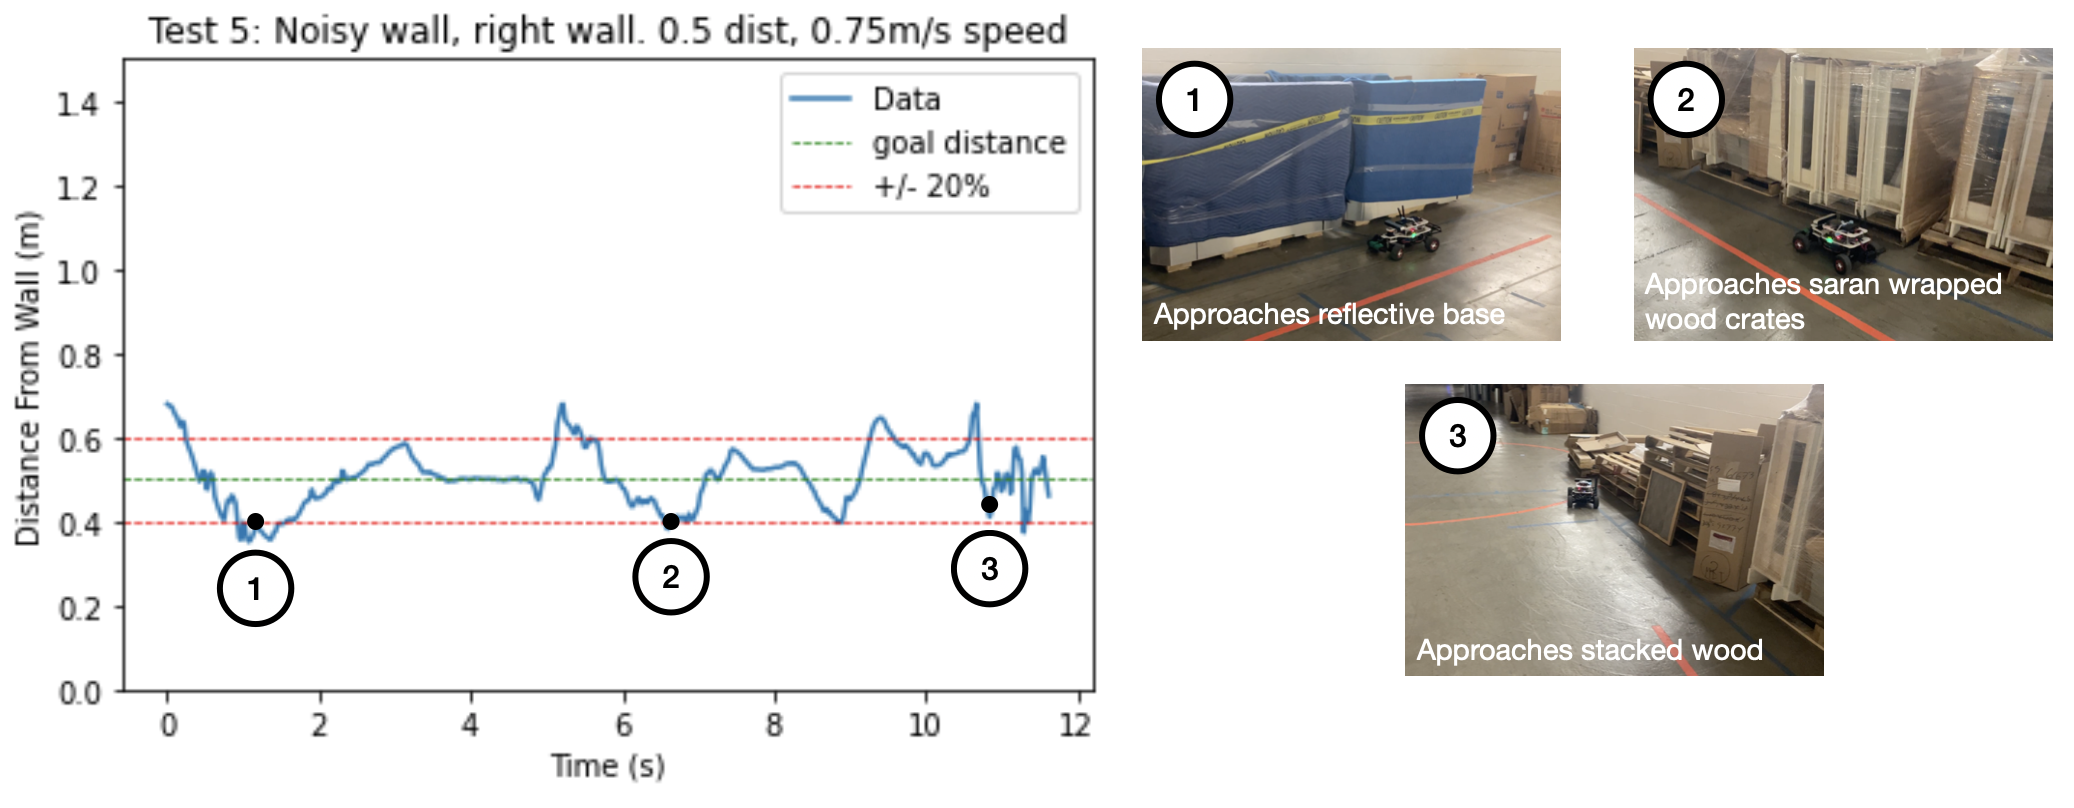
\includegraphics[width=0.8\textwidth]{noisy_figure.png} % Include the image placeholder.png
\caption{Wall Following: Noisy Surface}
\end{center}
\label{workflow}
\end{figure}

\subsection{Safety}
Our safety controller was activated in our Left Wall Following: Inner and Outer Corner test. The controller's behavior is shown in Figure 11. Here, we observed that as our car approaches and detects the pillar (an obstacle), our safety controller immediately stops sending commands to the controller, demonstrating robust safety performance.

\begin{figure}[H]
\begin{center}
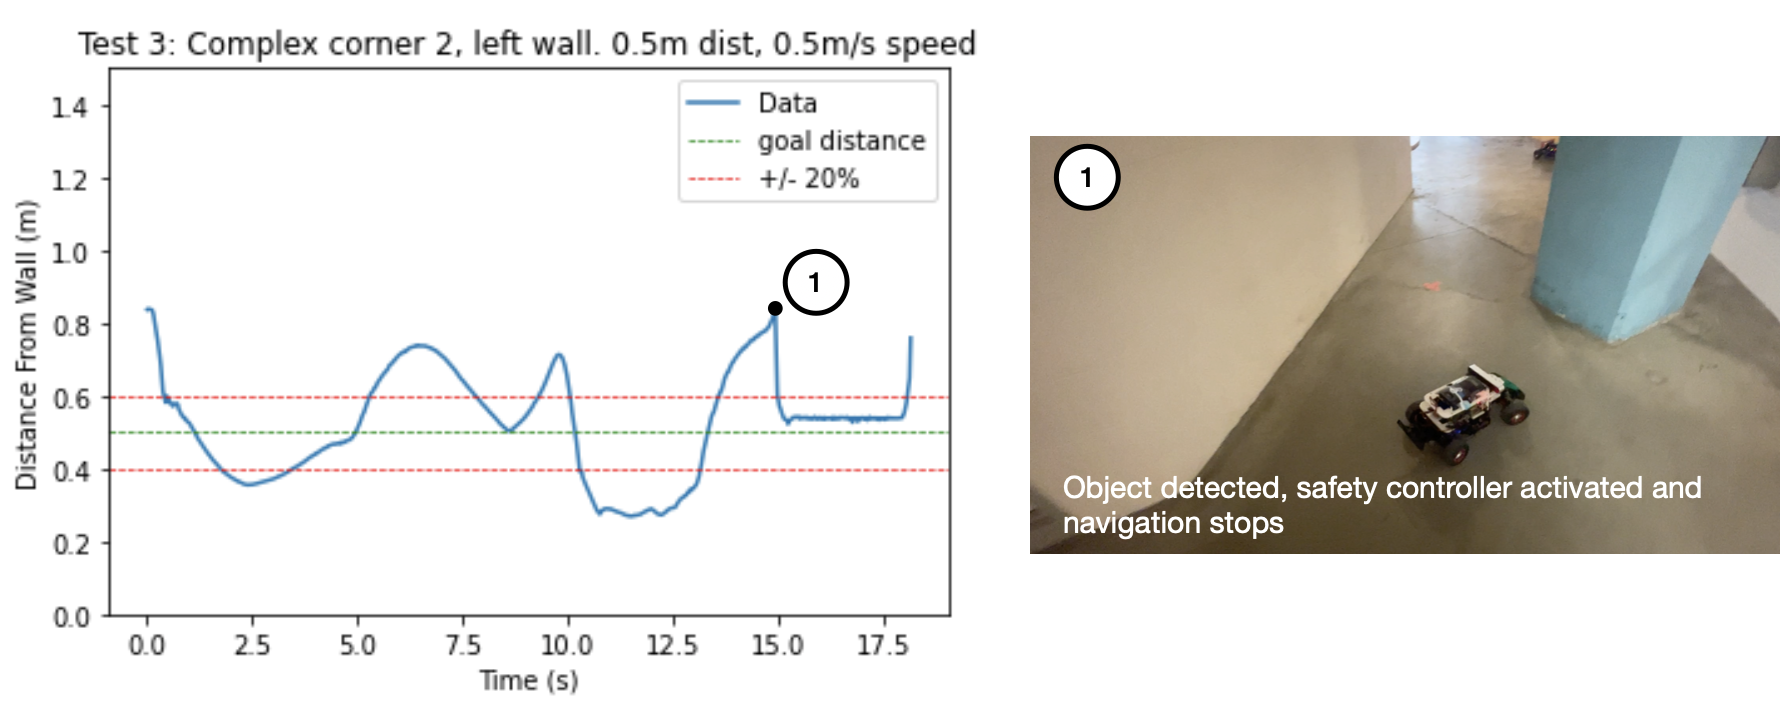
\includegraphics[width=0.8\textwidth]{safety_figure.png} % Include the image placeholder.png
\caption{Safety Controller Activation}
\end{center}
\label{workflow}
\end{figure}

\subsection{Link to Videos}

The below link can be used to access a dropbox with videos from various tests. The 5 tests discussed above with plots are labeled, the rest are in labeled subfolders. 
\begin{center} \href{https://www.dropbox.com/sh/i63v9yz40v15eeh/AACn9diRorBNhkWKkRiCIdyka?dl=0}{\underline{https://www.dropbox.com/sh/i63v9yz40v15eeh/AACn9diRorBNhkWKkRiCIdyka?dl=0}}
\end{center}

\section{Potential Improvements (Author: Steven Liu)}

While we are generally satisfied with the performance of our wall follower and safety controller, a number of improvements can certainly be made. Most obviously, while we did spend effort in tuning the gains and other variables to some degree, there is certainly room to tune them even further. This would likely involve extensive data processing in order to quantify the quality of the code; tuning as conducted was mostly visual in order to produce code that worked adequately as quickly as possible, without having to pause at each step of iteration to compute a number of evaluation metrics. \\

Corner detection and following could also clearly be improved. While our code can handle corners, overshoots are quite common. It is possible that this could be resolved simply by tuning existing our existing procedures to detect and react to corners, but it may also be the case that a high-quality corner follower would require more a more detailed procedure than is possible with simple linear regression and PID control. \\

The safety controller as implemented now is quite primitive. While it does account for the speed of the car, requiring more clearance for higher speeds, it does not account for other factors, such as the direction in which the car is trying to turn. It also has no mode in between no intervention and fully stopping, which can cause softlocks if the car gets stuck close to an obstruction, since the car will constantly be receiving instructions to stop regardless of what other nodes are doing. This can potentially be mitigated or resolved with intermediate modes, such as reducing the speed of the car instead of zeroing it out when it gets too close to an obstruction, or implementing a procedures to back away from obstructions so that the car can hopefully continue onward.

\section{Conclusion (Author: Jose Soto)}
% idea: this should prob be fairly high level overview of like everything, and steven can specifically talk in detail about potential improvements? if ur good w that bet 
This lab provided our team with a strong foundation in the hardware- which will prove invaluable in our future labs and the final assignment. The innovations and robustness present in our original code meant that were were successfully able to transition into the physical environment- only needing small adjustments to our wall-following algorithm and the implementation of a safety controller. We have completed our initial goal of creating a function wall following robot, and our testing reveals that both our wall following and safety systems are robust: working in a variety of test cases with variable speeds, amount of corners and large amounts of noise.   \\\\
We are still wary and very willing to revisit both these controller codes in future labs. We currently do not have a good idea for the specifications of the future labs- and our design philosophy for both of these controllers do not take these in account. We believe that there will be many improvements to our code specifically during the final implementation of our racing algorithm, as we anticipate there will be many optimizations as we try to make our car as fast and efficient as possible.  




\section{Lessons Learned}
%Presents individually authored self-reflections on technical, communication, and collaboration lessons you have learned in the course of this lab.

\subsection{Benjamin Rich}
I enjoyed the lab overall but learned a couple of useful things for the future. First, it seems like usually working on a lab in a group will be more productive than working individually on different parts and reconvening. It also seems like being very proactive on labs is ideal, as towards the end of a lab many groups want cars, hardware issues arise, etc. It was great getting to talk through the logic of different implementation approaches with team members!


\subsection{Dinuri Rupasinghe}
I enjoyed working on this lab. It was definitely helpful to work as a team to debug the robot. I found it very helpful when we found an effective, iterative way to debug. We often identified what problem we wanted to fix, and what aspects of our script and method could be causing it to error. We then chose to change one aspect of the script or method while keeping all else constant. This approach helped us better understand what was making our robot error. Overall, I really appreciated our team's workflow - we were able to allocate work where our strengths were while also taking turns learning more about what we were not familiar with.

\subsection{Sophia Wang}
Our group has a diverse set of skills, from hardware and programming debugging to data presentation, and I'm look forwarding to continuing this semester together. This lab assignment (implementing code from a previous lab onto the robot) was certainly an interesting transition into hardware workspaces and how simulation deviates from practice, however, I am even more excited to begin developing code as a team in the very near future. We were able to identify, just through simple testing in the basement, how future iterations in design would improve the autonomous system (e.g. computer vision for more robust obstacle detection, different feedback approaches, etc.) which was also a good exercise in the design cycle.

\subsection{Steven Liu}
My prior experience is certainly much more software-oriented; I've basically never written code that has been deployed to a machine with physical actuators. I'm not sure how much experience other people had, but having a group work on it together certainly made the task of learning how to operate the car much more manageable. This idea of learning things as a group being easier than trying to work through it as an individual is, I think, a valuable one to carry through to future labs. I think we've demonstrated that we can work together effectively to tinker with our designs and check each others' work.

\subsection{Jose Soto}
This lab was a great intro to the hardware- and I believe it was a very productive experience. I personally learned that starting our assignments early is essential in this class- as it's project-based and very open-ended and leads virtually infinite room for improvement (as well as, unfortunately, hardware mishaps). Additionally, this was the first time actually implementing a both a program and a control system on physical hardware, and I found it much easier than I expected. I'm very excited to employ our team's talent and creativity in the future labs, and especially the open-ended final design for our car.
\newpage 
\section{Appendix}

\subsection{Appendix A: PID Class Code}
\underline{Copy of PID Class Code. Language: Python 2.0}
{\footnotesize
\begin{verbatim}
import rospy

class PID:
    
    '''
    Basic PID Class
    Initialize with:
        - gains (kp, kd, ki)
        - setpoint (what to drive control to)
        - output limits (if wish to truncate control cmnds)
    '''

    def __init__(self,kp,kd,ki,setpoint,output_limits):
        
        '''
        Init, define useful class variables.
        '''

        self.kp = kp
        self.kd = kd 
        self.ki = ki
        self.setpoint = setpoint
        self.min_output = output_limits[0]
        self.max_output = output_limits[1]

        self.propLaw = 0 
        self.intLaw = 0
        self.derivLaw = 0

        self.last_time = rospy.Time.now()
        self.last_error = 0
        self.last_output = None
        self.last_input = None

    def changeParams(self, kpnew, kdnew, kinew, setpointnew):
        
        '''
        Change gains and setpoint if desired
        '''

        self.kp = kpnew; self.kd = kdnew; self.ki = kinew; self.setpoint = setpointnew
        return None
    

    def setInLimits(self, output, min, max):
        
        '''
        Mitigate output between [min,max] if desired. 
        '''
        
        if output < min:
            return min
        elif output > max:
            return max
        return output
    
    def control(self, input):
        
        '''
        Calculate error, calculate PID control, return control law
        input: current estimated state
        output: control output
        '''

        curr_time = rospy.Time.now()
        dt = (curr_time) - self.last_time # change in time
        dt = dt.to_sec() # convert to float
        error = self.setpoint - input 
        derror = error - self.last_error
        
        # see: https://en.wikipedia.org/wiki/PID_controller
        self.propLaw = self.kp * error
        self.intLaw = self.ki * (error+self.last_error)/2 * dt 
        self.derivLaw = self.kd * derror / dt 

        output = self.propLaw + self.intLaw + self.derivLaw 

        # update 
        self.last_output = output
        self.last_error = error
        self.last_input = input
        self.last_time = curr_time

        return output
\end{verbatim}
}
\subsection{Appendix B: Wall Follower Code}
\underline{Copy of Wall Follower Code. Language: Python 2.0}

{\footnotesize
\begin{verbatim}
#!/usr/bin/env python2

# GENERIC IMPORTS
import numpy as np
import rospy
from rospy.numpy_msg import numpy_msg
from sensor_msgs.msg import LaserScan
from ackermann_msgs.msg import AckermannDriveStamped
from std_msgs.msg import Header
from std_msgs.msg import Float32
from visualization_tools import *

# CUSTOM IMPORT
from PID import PID

class WallFollower:

    '''
    Wall Follower class. 
    Includes multiple methods for data manipulation. 

    Listens to /scan
    Publishes to nav/0 
    '''

    SCAN_TOPIC = rospy.get_param("wall_follower/scan_topic")
    DRIVE_TOPIC = rospy.get_param("wall_follower/drive_topic")
    SIDE = rospy.get_param("wall_follower/side")
    VELOCITY = rospy.get_param("wall_follower/velocity")
    DESIRED_DISTANCE = rospy.get_param("wall_follower/desired_distance")
    SIDE = rospy.get_param("wall_follower/side") # +1 left, -1 right
    WALL_TOPIC = "/wall"
    MAX_STEERING_ANGLE = 0.34

    def __init__(self): # init publisher and subscriber

        kp = 1; kd = .13; ki = 0.1 # INITIALIZE KP, KI, KD

        # INITIALIZE PID OBJECT
        self.PID = PID(kp,kd,ki,self.DESIRED_DISTANCE,(-1*self.MAX_STEERING_ANGLE, self.MAX_STEERING_ANGLE),self.VELOCITY)
        
        # INITALIZE PUBLISHERS / SUBSCRIBERS
        self.pubLaser = rospy.Publisher(self.DRIVE_TOPIC, AckermannDriveStamped, queue_size = 10)
        self.line_pub = rospy.Publisher(self.WALL_TOPIC, Marker, queue_size=1)
        self.minDistPub = rospy.Publisher('/mindist',Float32,queue_size = 10)
        rospy.Subscriber(self.SCAN_TOPIC, LaserScan, self.callback) # subscription topic name


    def sliceData(self, arr):

        '''
        Custom slicing method
            - Inputs: arr, array-like object
            - Outputs: (R,FR,FL,L), tuple of 4 lists, representing
            - right, forward right, forward left, and left data. 
        '''

        n = len(arr)
        start_ind = 0; end_ind = 0; found = False
        epsilon = 0.523599
        for i in range(n):
            if arr[i][1] > -np.pi/2-epsilon and not found:
                start_ind = i
                found = True
            if arr[i][1] >  np.pi/2+epsilon:
                end_ind = i
                break
        
        arr = arr[start_ind:end_ind+1]
        n = len(arr)
        portion = n//10
        return (arr[0:3*portion],arr[int(4.5*portion):5*portion],arr[5*portion:int(5.5*portion)], arr[7*portion:]) 
        # (right,frontright,frontleft,left)
    

    def PolarToRect(self, polarCoord):

        '''
        Conver polar coordinates (r,theta) to rectangular (x,y)
            - Input: polarCoord, a polar coordinate tuple of floats
            - Output: (x,y)
        '''

        x = polarCoord[0] * np.cos(polarCoord[1])
        y = polarCoord[0] * np.sin(polarCoord[1])
        return x, y
    

    def getMinAvgAllDist(self,x,y):

        '''
        Returns useful statistical data
            - Input: x,y two array-like objects of equal length
            - Output (minimum, avg, distances), min and avg
            - are ints, distances is array-like dist magnitudes
        '''

        new = np.sqrt(x**2+y**2)
        n = len(new); total = sum(new)
        return min(new), total/n, new
    

    def leastSquaresRegression(self,x,y):

        '''
        Peforms linear least squared regression.
            - Input: x,y; two array-like objects of equal length
            - Output; 
                - alpha: tuple, coeff of fitted line
                - predicted: array-like, predicted y-values of line
        '''

        A = np.vstack([x, np.ones(len(x))]).T
        y = y[:, np.newaxis]
        alpha = np.dot((np.dot(np.linalg.inv(np.dot(A.T,A)),A.T)),y)
        predicted = alpha[0]*x+alpha[1]
        return (alpha,predicted)
    
    
    def removeOutliers(self, x, y, gamma):

        '''
        Removes Outliers
            - Inputs:
                - x,y; array-like objects of equal length
                - gamma; float, if vals are
                  greater than min(|sqrt(x^2+y^2)|)*gamma 
                  they are removed
            - Output:
                - x_new, y_new; array-like objects of 
                  equal length with filtered data
        '''

        m, _, distances = self.getMinAvgAllDist(x,y)
        i_to_remove = []
        n = len(distances)
        for i in range(n):
            if distances[i] > gamma*m:
                i_to_remove.append(i)
        x_new = []; y_new = []
        for i in range(n):
            if i not in i_to_remove:
                x_new.append(x[i]); y_new.append(y[i])
        return np.array(x_new), np.array(y_new)


    def PolarToRectArray(self, arr):
        
        '''
        Converts array polar coordinates to rectangular coordinates 
            - Input: arr: array of polar coordinates (r,theta)
            - Outputs: xout, yout: array of rect coords
        '''

        xout = []; yout = []
        for val in arr:
            x , y = self.PolarToRect(val)
            xout.append(x); yout.append(y)
        xout = np.array(xout); yout = np.array(yout)
        return xout, yout


    def findWall(self, sliced, displayMarker, corner_threshold, constant_offset, gamma):

        '''
        Takes in sliced data, computes estimated distance using linear regression,
        filtering, etc. 
            - Inputs:
                - sliced: tuple of arrays, (R,FR,FL,L)
                - displayMarker: boolean, True if display marker in RVIZ
                - corner_threshold: float, if avg of 
                  min data is less than self.DESIRED_DISTANCE*corner_threshold
                  we assume robot is at a corner
                - constant_offset: float, to subtract from estimated distance if robot
                  is at a corner
                - gamma: float; see removeOutliers docs. 
            - Outputs:
                - alpha: tuple of floats, coeff for linear least squares model
                - predicted: array, predicted y-vals from lin regression
                - closest: estimated closest position with constant offset
                  applied if at a corner
        '''

        if self.SIDE == 1: # left
            wallData = sliced[-1]
            forwardMain, forwardSecondary = sliced[1], sliced[2]
        else: # right
            wallData = sliced[0]
            forwardMain, forwardSecondary = sliced[2], sliced[1]
        
        # CONVERT DATA FROM POLAR
        xValsWall, yValsWall = self.PolarToRectArray(wallData)
        xValsForward, yValsForward = self.PolarToRectArray(forwardMain)
        xValsForwardSec, yValsForwardSec = self.PolarToRectArray(forwardSecondary)

        # DETECT CORNER
        _, avg_dist, _ = self.getMinAvgAllDist(xValsForward,yValsForward)

        if avg_dist <= self.DESIRED_DISTANCE*corner_threshold:
            corner = True
            combined_x = np.concatenate((xValsForward, xValsWall, xValsForwardSec), axis=0) 
            # add in forward data if corner
            combined_y = np.concatenate((yValsForward, yValsWall, yValsForwardSec), axis=0) 
            # add in forward data if corner
        else:
            corner = False
            combined_x = xValsWall; combined_y = yValsWall # don't add in forward data if not corner

        combined_x, combined_y = self.removeOutliers(combined_x, combined_y, gamma)

        alpha,predicted = self.leastSquaresRegression(combined_x,combined_y) 
        closest, _, _ = self.getMinAvgAllDist(combined_x,predicted)

        if corner:
            closest -= constant_offset

        if displayMarker:
            VisualizationTools.plot_line(combined_x, predicted, self.line_pub, frame="/laser")

        return (alpha, predicted, closest)


    def createDriveObject(self, control):

        '''
        creates drive object
            - Input: control, value to set steering_angle to
            - Ouput: a, AckermannDrive object
        '''

        h = Header(); h.stamp = rospy.Time.now(); a = AckermannDriveStamped()
        a.header = h; a.drive.steering_angle = control; a.drive.speed = self.VELOCITY
        a.drive.acceleration = 0; a.drive.jerk = 0
        return a

    def callback(self, data): 

        '''
        Main Function. Takes in data, performs all necessary steps using helper function
        to publish a drive object such that the robot car follows a wall. 
            - Input: data, LaserScan object from /scan
            - Output: none, publishes AckermannDrive object
        '''

        # GET PUBLISHER
        publisher = self.pubLaser

        # GET LASERSCAN DATA
        DistAng = [] # array of (distance,angle)
        arrVals = np.array(data.ranges)
        minAng = data.angle_min
        angInc = data.angle_increment

        curr_ang = minAng
        for val in arrVals:
            DistAng.append((val,curr_ang))
            curr_ang += angInc

        sliced = self.sliceData(DistAng) # SLICE DATA
        # FIT LINE, GET PREDICTED VALUES AND CLOSEST VALUE
        _, _, closest = self.findWall(sliced, True, 2.5, .5, 2) 
        control = self.PID.control(closest) # GET CONTROL SIGNAL
        if self.SIDE == 1: # reverse control depending on law
            control *= -1
        publisher.publish(self.createDriveObject(control)) # CREATE AND PUBLISH DRIVE OBJECT
        mindistpub = self.minDistPub
        mindistpub.publish(closest)


if __name__ == "__main__":
    rospy.init_node('wall_follower')
    wall_follower = WallFollower()
    rospy.spin()

\end{verbatim}

}

\subsection{Appendix C: Safety Controller Code}
\underline{Copy of Safety Controller Code. Language: Python 2.0}

{\footnotesize
\begin{verbatim}
#!/usr/bin/env python2

import numpy as np

import rospy
from rospy.numpy_msg import numpy_msg
from sensor_msgs.msg import LaserScan
from ackermann_msgs.msg import AckermannDriveStamped
from visualization_msgs.msg import Marker
from visualization_tools import *
import tf2_ros

class SafetyController:
    
    '''
    SafetyController. Manges priorities and stops car if collision imminent. 
    Params:
        - User Params:
            - pause_time: float, amount of time to pause before moving.
                - if inf: never moves till node restarted
                - if 0: moves after obstacle removed
                - if x>0: moves at x seconds after obstacle removed
        - Other vars
            - min_dist: active update for minimum distance
            - paused: tracks if driving stopped
            - start_time: time of last time obstacle sensed
    '''

    # USER INPUTS:
    pause_time = 3.0 # seconds

    # ACTIVE STUFF
    min_dist = None 
    paused = False # tracks if driving commands are currently paused
    start_time = None # tracks start_time (time when pause command active)

    def __init__(self):
        
        '''
        Initialize publishers ans subscribers
        '''
        
        self.drive_pub = rospy.Publisher('/vesc/low_level/ackermann_cmd_mux/input/safety',AckermannDriveStamped,queue_size=10)
        rospy.Subscriber('/scan',LaserScan,self.read_laser_scan)
        rospy.Subscriber('/vesc/high_level/ackermann_cmd_mux/output',AckermannDriveStamped,self.check_drive_command)
        self.tfBuffer = tf2_ros.Buffer()
        self.listener = tf2_ros.TransformListener(self.tfBuffer)

    def read_laser_scan(self,data):

        '''
        Processes laserscan, extracts forwards data
            - Input: data, laserscan object
            - Output: None, updates self.min_dist 
        '''

        arrVals = np.array(data.ranges)
        portion = len(arrVals)/10.0
        forwards = arrVals[int(4*portion):int(6*portion)]
        self.min_dist = min(forwards)
    
    def check_drive_command(self,data):

        '''
        Callback function. Publishes drive command, modifies drive command so
        the car stops if a collission is imminent. 
            - Input: data, callback data
            - Output: none, publishes drive commnd
        '''

        if self.start_time != None:
            dt = (self.start_time - rospy.Time.now())
            dt = dt.to_sec()
        if self.paused and abs(dt) > self.pause_time:
            self.paused = False 

        if self.min_dist == None or self.min_dist < 0.15*data.drive.speed+0.30 or self.paused:
            drive_command = AckermannDriveStamped()
            drive_command.header.frame_id = 'base_link'
            drive_command.header.stamp = rospy.Time()
            drive_command.drive.speed = 0
            self.drive_pub.publish(drive_command)
            if not self.paused:
                self.paused = True
                self.start_time = rospy.Time.now()
            if self.min_dist == None or self.min_dist < 0.15*data.drive.speed+0.30:
                self.start_time = rospy.Time.now()
        else:
            self.drive_pub.publish(data)


if __name__ == "__main__":
    rospy.init_node('safety_controller')
    safety_controller = SafetyController()
    rospy.spin()

\end{verbatim}
}

\subsection{Appendix D: Rosbag Data Processing Code}
\underline{Copy of code used to Process Rosbag Outputs. Language: Python 3.0}
{\footnotesize
\begin{verbatim}
import numpy as np
import matplotlib.pyplot as plt
def loadDataRanges(file): #z = loadDataRanges('test1scan.txt')
    f = open(file, "r")
    data = [] # [[scan1ranges],[scan2ranges],...]
    count = 0
    for x in f:
        if count != 0:
            val = x.split(",")
            val = val[11:1092]
            data.append([float(x) for x in val])
        else:
            count += 1
    return data


def sliceData(arr):

    # custom slicing method, take svals close to side and on opposite side of front

    n = len(arr)
    start_ind = 0; end_ind = 0; found = False
    epsilon = 0.523599
    for i in range(n):
        if arr[i][1] > -np.pi/2-epsilon and not found:
            start_ind = i
            found = True
        if arr[i][1] >  np.pi/2+epsilon:
            end_ind = i
            break
    
    arr = arr[start_ind:end_ind+1]
    n = len(arr)
    portion = n//10
    # (right,frontright,frontleft,left)
    return (arr[0:3*portion],arr[int(4.5*portion):5*portion],arr[5*portion:int(5.5*portion)], arr[7*portion:]) 


def PolarToEuc(polarCoord):
    x = polarCoord[0] * np.cos(polarCoord[1])
    y = polarCoord[0] * np.sin(polarCoord[1])
    return x, y


def getMinAvgAllDist(x,y):
    new = np.sqrt(x**2+y**2)
    n = len(new); total = sum(new)
    return min(new), total/n, new


def leastSquaresRegression(x,y):
    # x,y are numpy arrays
    # returns ((coeff1,coeff2),[predicted vals])
    A = np.vstack([x, np.ones(len(x))]).T
    y = y[:, np.newaxis]
    alpha = np.dot((np.dot(np.linalg.inv(np.dot(A.T,A)),A.T)),y)
    predicted = alpha[0]*x+alpha[1]
    return (alpha,predicted)


def removeOutliers(x, y, gamma):
    # removes outliers more than gamma*MIN_DIST
    m, _, distances = getMinAvgAllDist(x,y)
    i_to_remove = []
    n = len(distances)
    for i in range(n):
        if distances[i] > gamma*m:
            i_to_remove.append(i)
    x_new = []; y_new = []
    for i in range(n):
        if i not in i_to_remove:
            x_new.append(x[i]); y_new.append(y[i])
    return np.array(x_new), np.array(y_new)


def PolarToEucArray(arr):
    # arr: (dist,ang)
    # returns: two numpy arrays, x & y
    xout = []; yout = []
    for val in arr:
        x , y = PolarToEuc(val)
        xout.append(x); yout.append(y)
    xout = np.array(xout); yout = np.array(yout)
    return xout, yout


def findWall(SIDE, sliced, corner_threshold, gamma,DESIRED_DISTANCE):

    if SIDE == 1: # left
        wallData = sliced[-1]
        forwardMain, forwardSecondary = sliced[1], sliced[2]
    else: # right
        wallData = sliced[0]
        forwardMain, forwardSecondary = sliced[2], sliced[1]
    
    # CONVERT DATA FROM POLAR
    xValsWall, yValsWall = PolarToEucArray(wallData)
    xValsForward, yValsForward = PolarToEucArray(forwardMain)
    xValsForwardSec, yValsForwardSec = PolarToEucArray(forwardSecondary)

    # DETECT CORNER
    _, avg_dist, _ = getMinAvgAllDist(xValsForward,yValsForward)

    combined_x = xValsWall; combined_y = yValsWall # don't add in forward data if not corner

    combined_x, combined_y = removeOutliers(combined_x, combined_y, gamma)

    alpha,predicted = leastSquaresRegression(combined_x,combined_y) 
    closest, _, _ = getMinAvgAllDist(combined_x,predicted)

    return (alpha, predicted, closest)


###########################################

def reject_outliers(data, m = 2.):
    d = np.abs(data - np.median(data))
    mdev = np.median(d)
    s = d/mdev if mdev else np.zero(len(d))
    out = []
    return data[s<m]

def mainFunc(fileName,wall,DESIRED_DISTANCE,angle_min,angle_increment):
    allData = loadDataRanges(fileName)
    distance_from_wall = []
    for timestep in allData:
        DistAng = [] # array of (distance,angle)
        curr_ang = angle_min
        for val in timestep:
            DistAng.append((val,curr_ang))
            curr_ang += angle_increment
        sliced = sliceData(DistAng) # SLICE DATA
        _, _, closest = findWall(wall, sliced, 2.5, 2, DESIRED_DISTANCE) # FIT LINE, GET PREDICTED VALUES AND CLOSEST VALUE
        distance_from_wall.append(closest)
    if fileName == "test1scan.txt":
        return distance_from_wall
    return reject_outliers(np.array(distance_from_wall))

def secoFunc(fileName,wall,DESIRED_DISTANCE,angle_min,angle_increment):
    allData = loadDataRanges(fileName)
    distance_from_wall = []
    for timestep in allData:
        distance_from_wall.append(min(timestep))
    return reject_outliers(np.array(distance_from_wall), m=2.)

def computeError(data,setpoint):
    data = np.array(data)
    return data-setpoint

print('processing data...')
test1 = mainFunc("test1scan.txt",-1,0.5,-2.35619449615,0.00436332309619)
test1err = computeError(test1,0.5)
test2 = mainFunc("test2scan.txt",-1,0.5,-2.35619449615,0.00436332309619)
test2err = computeError(test2,0.5)
test3 = mainFunc("test3scan.txt",1,0.5,-2.35619449615,0.00436332309619)
test3err = computeError(test3,0.5)
test4 = mainFunc("test4scan.txt",-1,0.75,-2.35619449615,0.00436332309619)
test4err = computeError(test4,0.75)
test5 = mainFunc("test5scan.txt",-1,0.5,-2.35619449615,0.00436332309619)
test5err = computeError(test5,0.5)


t_init = 0
t1 = []
for i in range(len(test1)):
    t1.append(t_init)
    t_init += .0251 # seconds, estimated
t_init = 0
t2 = []
for i in range(len(test2)):
    t2.append(t_init)
    t_init += .0251 # seconds, estimated
t_init = 0
t3 = []
for i in range(len(test3)):
    t3.append(t_init)
    t_init += .0251 # seconds, estimated
t_init = 0
t4 = []
for i in range(len(test4)):
    t4.append(t_init)
    t_init += .0251 # seconds, estimated
t_init = 0
t5 = []
for i in range(len(test5)):
    t5.append(t_init)
    t_init += .0251 # seconds, estimated

print('done!')
print('plotting...')

plt.figure(1)
plt.title('Test 1: Flat wall, angled start, right wall. 0.5m dist, 0.5m/s speed')
plt.plot(t1,test1, label = 'Data')
plt.axhline(y = 0.5, color = 'g', linestyle = 'dashed', label = 'goal distance', linewidth='.7')
plt.axhline(y = 0.5*.8, color = 'r', linestyle = 'dashed', label = '+/- 20%', linewidth='.7')
plt.axhline(y = 0.5*1.2, color = 'r', linestyle = 'dashed', linewidth='.7')
plt.legend()
plt.xlabel('Time (s)')
plt.ylabel('Distance From Wall (m)')
plt.ylim(0,2)
plt.show()

plt.figure(3)
plt.title('Test 2: Complex multi-corner, right wall. 0.5m dist, 0.5m/s speed')
plt.plot(t2,test2, label = 'Data')
plt.axhline(y = 0.5, color = 'g', linestyle = 'dashed', label = 'goal distance', linewidth='.7')
plt.axhline(y = 0.5*.8, color = 'r', linestyle = 'dashed', label = '+/- 20%', linewidth='.7')
plt.axhline(y = 0.5*1.2, color = 'r', linestyle = 'dashed', linewidth='.7')
plt.legend()
plt.xlabel('Time (s)')
plt.ylabel('Distance From Wall (m)')
plt.ylim(0,1.5)
plt.show()

plt.figure(5)
plt.title('Test 3: Complex corner 2, left wall. 0.5m dist, 0.5m/s speed')
plt.plot(t3,test3, label = 'Data')
plt.axhline(y = 0.5, color = 'g', linestyle = 'dashed', label = 'goal distance', linewidth='.7')
plt.axhline(y = 0.5*.8, color = 'r', linestyle = 'dashed', label = '+/- 20%', linewidth='.7')
plt.axhline(y = 0.5*1.2, color = 'r', linestyle = 'dashed', linewidth='.7')
plt.legend()
plt.xlabel('Time (s)')
plt.ylabel('Distance From Wall (m)')
plt.ylim(0,1.5)
plt.show()

plt.figure(7)
plt.title('Test 4: Complex corner, right wall. 0.75m dist, 1.5m/s speed')
plt.plot(t4,test4, label = 'Data')
plt.axhline(y = 0.75, color = 'g', linestyle = 'dashed', label = 'goal distance', linewidth='.7')
plt.axhline(y = 0.75*.8, color = 'r', linestyle = 'dashed', label = '+/- 20%', linewidth='.7')
plt.axhline(y = 0.75*1.2, color = 'r', linestyle = 'dashed', linewidth='.7')
plt.legend()
plt.xlabel('Time (s)')
plt.ylabel('Distance From Wall (m)')
plt.ylim(0,1.5)
plt.show()

plt.figure(9)
plt.title('Test 5: Noisy wall, right wall. 0.5 dist, 0.75m/s speed')
plt.plot(t5,test5, label = 'Data')
plt.axhline(y = 0.5, color = 'g', linestyle = 'dashed', label = 'goal distance', linewidth='.7')
plt.axhline(y = 0.5*.8, color = 'r', linestyle = 'dashed', label = '+/- 20%', linewidth='.7')
plt.axhline(y = 0.5*1.2, color = 'r', linestyle = 'dashed', linewidth='.7')
plt.legend()
plt.xlabel('Time (s)')
plt.ylabel('Distance From Wall (m)')
plt.ylim(0,1.5)
plt.show()

print('done!')
\end{verbatim}
}























% \section{Formatting examples for figures, pseudocode, etc}

% \subsection{Tables}

% Many other table packages and options exist but here is one example:\\\\

% \begin{tabularx}{0.8\textwidth} {
%   | >{\raggedright\arraybackslash}X
%   | >{\centering\arraybackslash}X
%   | >{\raggedleft\arraybackslash}X | }
%  \hline
%  item 11 & item 12 & item 13 \\
%  \hline
%  item 21  & item 22  & item 23  \\
% \hline
% \end{tabularx}

% \subsection{Images}

% \begin{figure}[h]
% \begin{center}
% \includegraphics[width=0.65\textwidth]{placeholder} % Include the image placeholder.png
% \caption{Figure caption.}
% \end{center}
% \end{figure}

% \subsection{Code Blocks and Algorithm Pseudocode}

% % Including Python code blocks:

% \begin{lstlisting}
% json
% {
%   "6.141": "normal",
%   "16.405": "woke",
%   "no_sleep": "spoke"
% }

% def do_something_productive():
%   if not_productive:
%     do_work()
%   else:
%     cry()
% \end{lstlisting}

% % Using the algorithm2e package for pseudocode:

% \begin{algorithm}[H]
% \SetAlgoLined
%  \While{alive}{
%   \eIf{sleepy}{
%    sleep\;
%    }{
%    eat\;
%   }
%  }
%  \caption{caption}
% \end{algorithm}

% % Using the algorithmic package for pseudocode:

% \begin{algorithmic}
% \STATE $i\gets 10$
% \IF {$i\geq 5$}
%         \STATE $i\gets i-1$
% \ELSE
%         \IF {$i\leq 3$}
%                 \STATE $i\gets i+2$
%         \ENDIF
% \ENDIF
% \end{algorithmic}



% \textbf{Notes from Lec 3/6/2022}
% Things to consider:
% \begin{enumerate}
%     \item what does a holistic evaluation look like? A: qualitataive and quantitative 
%     \item Objective metrics? what percent does it stay within some bounds, distance from rosbag
%     \item Intrinsic Metrics? how often does it accomplish goal.
%     \item Qualitative observations ; it works.  How much overshoot does it have? 
%     \item Vulnerabilities? See through wall (window), non-corner obstacles (i.e. column), cuts in wall that are shallow (treats as a corner) 
%     \item Robustness? robust to different speeds, different distances from wall, l/r wall, robust to disturbances and noise. Vulnerability to cornering at high speed low distance. Not tested on curvd walls. 
% \end{enumerate}

\end{document}